\documentclass[../main.tex]{subfiles}
\graphicspath{{\subfix{../imagenes/}}}

\begin{document}

\chapter{Conclusions} \label{chap:conclusions} 
    

    Through this experimental setup, we assessed how well our continual learning process improves our system's performance over time. This directly demonstrates the adaptive capabilities of our system, showing its ability to mature and refine its performance in response to new data.

     By demonstrating the effectiveness of these tactics, we aim to devise a reliable and self-improving system capable of continuously enhancing its performance and capability to cater to evolving datasets and real-world scenarios, thus maximizing its usefulness in TB diagnosis.
    
    \todo[inline]{Discuss the results obtained and implications in the project context, limitations of the proposed system, future work, etc.}
    
    \improvement[inline]{sobretodo habla de los objetivos alcanzados y los no alcanzados, habla de como los resultados  validan que tu sistema es bueno por..}


     \improvement[inline]{no se si esta muy clara la diferencia entre trabajo futuro y futuras lineas de investigacion. Esta bien, puedes proponer nuevas ideas y direcciones pero no lo conviertas en un estado del arte tocando todas las posibles direcciones.}
     

    \section{Main Implications} \label{conclusions:implications} \info{0.65 pág}

    \section{Limitations of the System} \label{conclusions:limitations} \info{0.5 pág}
    
    \section{Future Work} \label{conclusions:future_work} \info{~2.75 pág}
    % \addcontentsline{toc}{section}{Future Work}

    The following section\dots

    \subsection{
        Implementing new adaptation strategies to the system 
    } \label{conclusions:future_work:adaptation_strategies}\info{0.5 pág}


    \subsection{
        Improving the explainability of the continual learning process 
    }   \label{conclusions:future_work:explainability}\info{0.5 pág}
    \improvement{no se si esto lo pondría en limitaciones} 
    
    Anytime a model is trained on a particular dataset, any biases present on that dataset are also introduced to the model. In any high-stakes environment, the researchers who design these models should be aware of the biases present in the data and how they might affect the model's predictions and consider them in the decision-making process.

    % quito este parrafo porque igual no aporta mucho, tienes razón que lo hace parecer como otro Estado del arte
    
    % Furthermore, this aspect is especially crucial in the healthcare sector, where legislation and ethical guidelines stress the importance of AI systems being transparent \cite{noauthor_ethics_2019,eu_aiact_2023}. Healthcare professionals have the moral and legal obligation to be able to explain the decisions made by the AI systems they use to the relevant stakeholders, and the latter also has the right to know how the decisions that affect them are made.
    
    In that regard, one of the main limitations of the system proposed here is the lack of explainability of the continual learning process, where a model that is designed initially to be as transparent as possible might gradually lose explainability power as it adapts to new data distributions over time.
    
    Methods such as TRAK \cite{park_trak_2023} have been proposed as a way to improve the explainability of DNNs by providing a way to trace the predictions of a model to individual instances of their training data in a concept known as \textit{data attribution}, which has been proven helpful in improving sample selection for active learning approaches \cite{park_trak_2023, holzmuller_framework_2023, liu_influence_2021}.

    \subsection{Potential to run the system as a federated learning platform} \label{conclusions:future_work:federated} \info{1.75 pág}

    % \info{1 page}

    Federated learning is the concept of training a model using data from multiple sources without having to share the data itself. This is achieved by training the model on each source separately and combining the results to obtain a final model. 
    
    Efforts such as Joshi et al.'s (2022) \cite{joshi_federated_2022} have demonstrated the benefits and potential of taking a federated learning approach to training machine learning models in the healthcare industry to protect the privacy of patients and/or give more utility to highly-valuable datasets that might require significant research effort to collect.
    
    Thus, a future we envision to improve the system presented in this work would be to propose a federated system where multiple research units train an instance of a global model - previously agreed to be trained  - with its own local data and share the trained weights with a central server. 
    
    Each client could have an instance of the same annotation frontend and backend system we developed in this thesis, including the active learning framework running locally with their own data. 
    
    The motivation for this comes from the fact that it is challenging to convince partners (even within the same project organization) to share their data. In the healthcare industry, data is considered a very valuable asset, with a high cost to obtain and annotate, which is why it is often used as a bargaining chip in negotiations between companies and research organizations \todo{include citation}.

    Figure \ref{fig:federated} illustrates the concept of a federated learning system:

    \begin{figure}
        \centering
        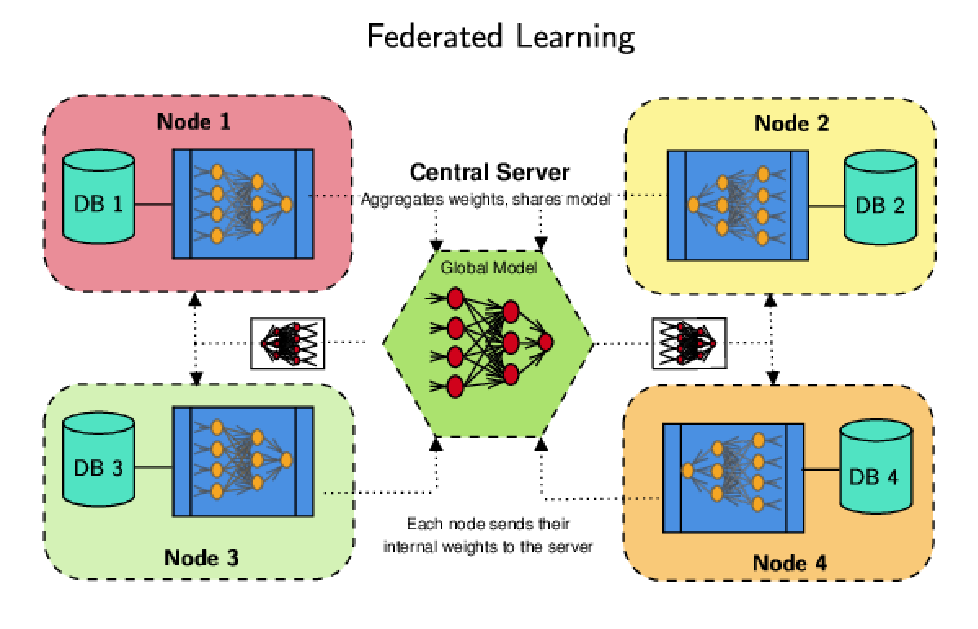
\includegraphics[width=0.85\linewidth]{figures/federated.pdf}
        \caption{Illustration of a Federated Learning System}
        \label{fig:federated}
    \end{figure}
    

    \todo[inline]{Show a diagram of the proposed federated learning system.}

    % \clearpage

    \subsection{Comments on Further Research Directions} \label{conclusions:research_directions}

    We made a relatively lengthy discussion of other topics tangential to the ideas dealth in this thesis that we consider to be interesting potential for further research. This discussion is presented in \nameref{appendix:further_research}, as to not distract from the content in this chapter that is more relevant to the project we worked on. 

    Unlike the previous section, which focused on the limitations of the proposed system and detailed ideas about how to address or improve them in the immediate future, this section takes a broader view, focusing on gaps in the current state-of-the-art and what might be considered to be the next steps in the field.
    

    \section{Final Remarks} \label{conclusions:final_remarks} \info{0.75 pág}
    
    \dots

    Unlike many scientific advances, breakthroughs such as a true self-improving model that adapts itself continually in an online fashion will have immediate applications in every domain, from healthcare to education, to economics, to scientific discovery itself \dots 

% \printbibliography
\end{document}